\chapter{Casi d'uso}\label{CasiDUso}
In questo capitolo vengono elencati i casi d'uso$_G$ individuati per il progetto \textit{GDP: Gathering Detection Platform} in accordo con il proponente$_{\scaleto{G}{3pt}}$. Ogni caso d'uso$_{\scaleto{G}{3pt}}$ indica un'interazione tra uno o più attori e il sistema. Questa interazione genera uno scenario, cioè l'insieme delle azioni che hanno in comune uno scopo finale per un attore. I casi d'uso$_{\scaleto{G}{3pt}}$ vengono identificati nel seguente modo:
\begin{center}
	\textbf{UC[codice\_Padre].[codice\_Figlio]}
\end{center}
La descrizione della classificazione è la seguente:
\begin{itemize}
	\item \textbf{UC}: acronimo per User Case$_G$, parola inglese che si traduce in Casi D'uso$_{\scaleto{G}{3pt}}$;
	\item \textbf{Codice\_Padre.Codice\_Figlio}: codice univoco per ogni caso d'uso$_{\scaleto{G}{3pt}}$ nella forma gerarchica padre/figlio.
\end{itemize}

\section{Casi d'uso tra un utente e il front end}\label{CasiDUsoCasiDUsoTraUnUtenteEIlFrontEnd}
%spiegazione della sezione
\subsection{Attori dei casi d'uso}\label{CasiDUsoCasiDUsoTraUnUtenteEIlFrontEndAttoriDeiCasiDUso}
\begin{center}
	\begin{figure}[H]
		
\includegraphics{../immagini/attori_casi/utente_generico.png}
		\caption{Attore: utente generico}
	\end{figure}
\end{center}
\subsubsection{Attori Primari}\label{CasiDUsoCasiDUsoTraUnUtenteEIlFrontEndAttoriDeiCasiDUsoAttoriPrimari}
\begin{itemize}
	\item \textbf{Utente generico:} definisce l'utente generico che utilizza l'applicazione web.
\end{itemize}

\subsection{Elenco casi d'uso}\label{CasiDUsoCasiDUsoTraUnUtenteEIlFrontEndElencoCasiDUso}

\begin{center}
	\begin{figure}[H]
		\centering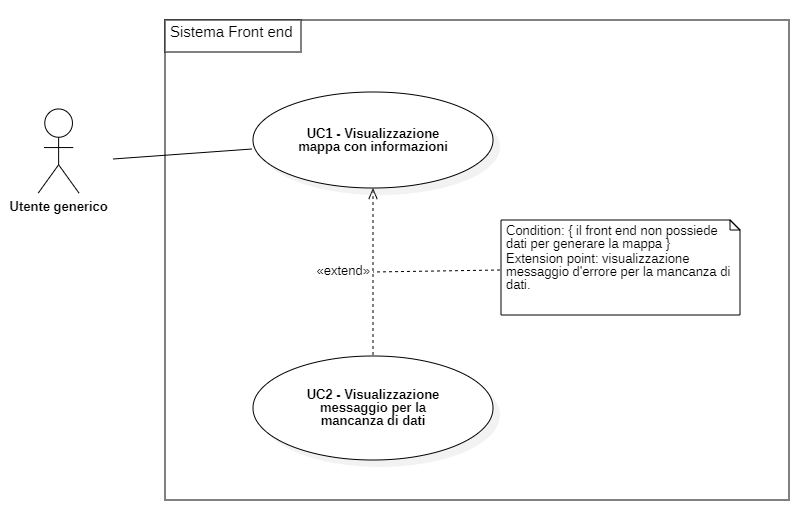
\includegraphics[scale=0.8]{../immagini/attori_casi/UC_1_2.png}
		\caption{Schema generale visualizzazione mappa con errori annessi}
	\end{figure}
\end{center}

\subsubsection{UC1 - Visualizzazione informazioni sulla mappa}\label{CasiDUsoCasiDUsoTraUnUtenteEIlFrontEndElencoCasiDUsoUC1VisualizzazioneInformazioniSullaMappa} %parzialmente corretto


\begin{itemize}
	\item \textbf{Attori primari}: utente generico;
	\item \textbf{Descrizione}: l’utente accede all’applicazione web e visualizza la heat map$_{\scaleto{G}{3pt}}$. La mappa mostra la città impostata di default o quella selezionata tra quelle a disposizione, come definito nell’UC8(sezione \ref{CasiDUsoCasiDUsoTraUnUtenteEIlFrontEndElencoCasiDUsoUC4SelezioneCittaDaVisualizzareNellaMappa}). Le informazioni vengono ricavate dall’orario e la data impostate dall’utente come indicato nel UC9.1(sezione \ref{CasiDUsoCasiDUsoTraUnUtenteEIlFrontEndElencoCasiDUsoUC51SelezioneDellOrario}) e UC9.2(sezione \ref{CasiDUsoCasiDUsoTraUnUtenteEIlFrontEndElencoCasiDUsoUC52ModificaDellaData}) o si utilizzano i dati in tempo reale quindi usando l’orario attuale;
	\item \textbf{Scenario principale}: L’utente accede all’applicazione web e visualizza la heat map$_{\scaleto{G}{3pt}}$ della città;
	\item \textbf{Precondizione}: il front end$_{\scaleto{G}{3pt}}$ può generare la mappa; la città, la data, l’ora sono state indicate dall’utente, seguendo quanto descritto rispettivamente nell'UC8 (sezione \ref{CasiDUsoCasiDUsoTraUnUtenteEIlFrontEndElencoCasiDUsoUC4SelezioneCittaDaVisualizzareNellaMappa}), nell'UC9.2(sezione \ref{CasiDUsoCasiDUsoTraUnUtenteEIlFrontEndElencoCasiDUsoUC52ModificaDellaData}) e nell'UC9.1(sezione \ref{CasiDUsoCasiDUsoTraUnUtenteEIlFrontEndElencoCasiDUsoUC51SelezioneDellOrario}), o vengono utilizzate quelle di default, quindi data e ora sono quelle odierne di sistema per dati in tempo reale e la città è quella impostata di default;
	\item \textbf{Postcondizione}: l’utente visualizza la heat map$_{\scaleto{G}{3pt}}$ con i dati ricavati nell’istante di tempo selezionato, come definito nell’UC9 (sezione \ref{CasiDUsoCasiDUsoTraUnUtenteEIlFrontEndElencoCasiDUsoUC5SelezioneDellIstanzeDiCuiVisualizzareIDatiNellaHeatmap}), e alla città scelta fra quelle disponibili come descritto nella definizione dell’UC8 (sezione \ref{CasiDUsoCasiDUsoTraUnUtenteEIlFrontEndElencoCasiDUsoUC4SelezioneCittaDaVisualizzareNellaMappa});
	\item \textbf{Estensioni}: l’utente accede all’applicazione web, il front end$_{\scaleto{G}{3pt}}$, rilevando la richiesta di generazione della mappa, individua una mancanza di dati per la sua costruzione e di conseguenza viene visualizzato un messaggio relativo all’errore riscontrato (UC2, sezione \ref{CasiDUsoCasiDUsoTraUnUtenteEIlFrontEndElencoCasiDUsoUC2VisualizzazioneMessaggioPerLaMancanzaDiDati});
\end{itemize}

\subsubsection{UC2 - Visualizzazione messaggio per la mancanza di dati }\label{CasiDUsoCasiDUsoTraUnUtenteEIlFrontEndElencoCasiDUsoUC2VisualizzazioneMessaggioPerLaMancanzaDiDati} %parzialmente corretto
\begin{itemize}
	\item \textbf{Attori primari}: utente generico;
	\item \textbf{Descrizione}: l’utente visualizza un  ’errore per la mancanza di dati necessari alla generazione della mappa. Questo accade quando il front end$_{\scaleto{G}{3pt}}$ non ha a disposizione tutti i dati;
	\item \textbf{Scenario principale}:
	\begin{itemize}
		\item l’operazione di generazione mappa fallisce;
		\item l’utente visualizza un errore per la mancanza dei dati;
		\item l’utente clicca il pulsante “ok” per chiudere il messaggio.
	\end{itemize}
	\item \textbf{Precondizione}: il front end$_{\scaleto{G}{3pt}}$ effettua un controllo sui dati, non sono presenti tutti i dati;
	\item \textbf{Postcondizione}: viene visualizzato un messaggio all’utente per informarlo sul problema riscontrato e l’operazione fallisce.
\end{itemize}


\begin{center}
	\begin{figure}[H]
		\centering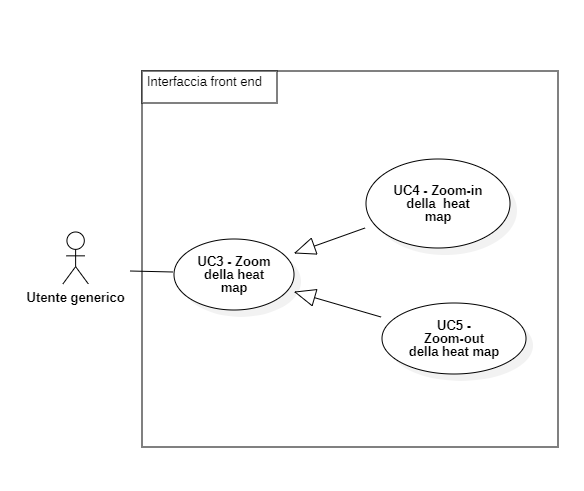
\includegraphics[scale=0.8]{../immagini/attori_casi/UC_3_4_5.png}
		\caption{Schema generale zoom della heat-map$_{\scaleto{G}{3pt}}$}
	\end{figure}
\end{center}


\subsubsection{UC3 - Zoom della heat map}\label{CasiDUsoCasiDUsoTraUnUtenteEIlFrontEndElencoCasiDUsoUC3ZoomDellaHeatMap}

Dopo un'attenta analisi, il gruppo ha deciso di porre questo caso d'uso separato rispetto all'UC1 (sezione \ref{CasiDUsoCasiDUsoTraUnUtenteEIlFrontEndElencoCasiDUsoUC1VisualizzazioneInformazioniSullaMappa}) con lo scopo di renderlo disponibile per una possibile mappa differente da quella presente.



\begin{itemize}
	\item \textbf{Attori primari:} utente generico;
	\item \textbf{Descrizione:} l’utente, durante la visualizzazione della heat map$_{\scaleto{G}{3pt}}$, può variare il livello di zoom della mappa della città selezionata attraverso l'interfaccia;
	\item \textbf{Scenario principale:} l’utente attraverso l'interfaccia può decidere di modificare il livello di zoom della mappa visualizzata;
	\item \textbf{Generalizzazioni:}\begin{enumerate}
		\item UC4 - Zoom-in della heat map$_{\scaleto{G}{3pt}}$;
		\item UC5 - Zoom-out della heat map$_{\scaleto{G}{3pt}}$.
	\end{enumerate}
	\item \textbf{Precondizione:} il sistema è funzionante e la mappa è stata caricata;
	\item \textbf{Postcondizione:} il livello di zoom della mappa è aumentato o diminuito in base all'azione che compie l'utente.
\end{itemize}

\subsubsection{UC4 - Zoom-in della heat map}\label{CasiDUsoCasiDUsoTraUnUtenteEIlFrontEndElencoCasiDUsoUC31ZoomInDellaHeatMap}

\begin{itemize}
	\item \textbf{Attori primari:} utente generico;
	\item \textbf{Descrizione:} l’utente, durante la visualizzazione della heat map$_{\scaleto{G}{3pt}}$, può aumentare il livello di zoom per vedere in dettaglio la mappa della città selezionata;
	\item \textbf{Scenario principale:} l’utente aumenta il livello di zoom della heat map$_{\scaleto{G}{3pt}}$ per una visualizzazione dettagliata della città, dopo aver compiuto questa azione l'utente inoltre può: spostarsi all'interno della mappa (UC6, sezione \ref{CasiDUsoCasiDUsoTraUnUtenteEIlFrontEndElencoCasiDUsoUC311SpostamentoDelCentroDellaMappa}) e visualizzare le etichette (denonimate pop-up$_G$) dei punti di interesse (UC7, sezione \ref{CasiDUsoCasiDUsoTraUnUtenteEIlFrontEndElencoCasiDUsoUC312VisualizzazioneDelPopupDiUnPuntoDiInteresse});
	\item \textbf{Precondizione:} il sistema dispone di informazioni relative alla città e il livello di zoom-in non è al massimo;
	\item \textbf{Postcondizione:} la heat map$_{\scaleto{G}{3pt}}$ si aggiorna mostrando livelli di informazioni più dettagliate in base al livello di zoom in effettuato.
\end{itemize}

\subsubsection{UC5 - Zoom-out della heat map}\label{CasiDUsoCasiDUsoTraUnUtenteEIlFrontEndElencoCasiDUsoUC32ZoomOutDellaHeatMap}

\begin{itemize}
	\item \textbf{Attori primari:} utente generico;
	\item \textbf{Descrizione:} l’utente, durante la visualizzazione della heat map$_{\scaleto{G}{3pt}}$, può diminuire il livello di zoom per vedere informazioni meno dettagliate della città selezionata;
	\item \textbf{Scenario principale:} l’utente diminuisce il livello di zoom della heat map$_{\scaleto{G}{3pt}}$ per una visualizzazione meno dettagliata della città;
	\item \textbf{Precondizione:}  il sistema dispone di informazioni relative alla città e il livello di zoom-out non è al massimo;
	\item \textbf{Postcondizione:} la heat map$_{\scaleto{G}{3pt}}$ si aggiorna mostrando livelli di informazioni meno dettagliate in base al livello di zoom-out effettuato.
\end{itemize}

\begin{center}
	\begin{figure}[H]
		\centering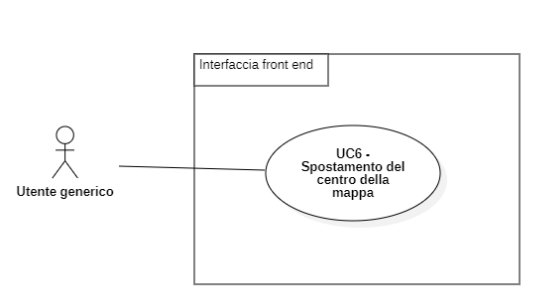
\includegraphics[scale=0.8]{../immagini/attori_casi/UC_6.png}
		\caption{Schema generale spostamento della mappa}
	\end{figure}
\end{center}


\subsubsection{UC6 - Spostamento all'interno della mappa}\label{CasiDUsoCasiDUsoTraUnUtenteEIlFrontEndElencoCasiDUsoUC311SpostamentoDelCentroDellaMappa}

\begin{itemize}
	\item \textbf{Attori primari:} utente generico;
	\item \textbf{Descrizione:} l’utente può spostarsi all’interno della mappa, utilizzando il cursore può trascinare la mappa nel punto che vuole visualizzare;
	\item \textbf{Scenario principale:} l'utente decide di visualizzare un punto diverso da quello di default, presentato nella mappa, e quindi trascinandola si sposta per osservarlo;
	\item \textbf{Precondizione:} il livello di zoom-in$_{\scaleto{G}{3pt}}$ è diverso da quello iniziale e si sta visualizzando la mappa nelle coordinate della città scelta o impostasta di default;
	\item \textbf{Postcondizione:} visualizza la mappa in un punto diverso rispetto al punto di partenza.
\end{itemize}

\begin{center}
	\begin{figure}[H]
		\centering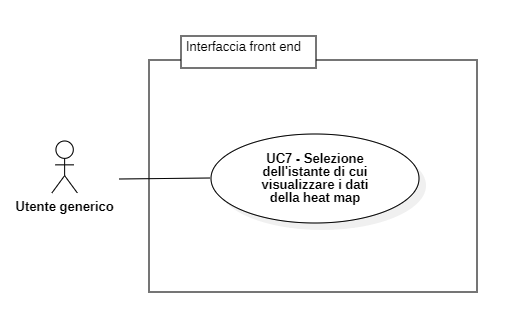
\includegraphics[scale=0.8]{../immagini/attori_casi/UC_7.png}
		\caption{Schema generale visualizzazione delle informazioni nell'etichetta}
	\end{figure}
\end{center}


\subsubsection{UC7 - Visualizzazione delle informazioni nell'etichetta del punto di interesse}\label{CasiDUsoCasiDUsoTraUnUtenteEIlFrontEndElencoCasiDUsoUC312VisualizzazioneDelPopupDiUnPuntoDiInteresse}

\begin{itemize}
	\item \textbf{Attori primari:} utente generico;
	\item \textbf{Descrizione:} l’utente visualizza un'icona del punto di interesse. All'icona è associata un'etichetta contenente le informazioni riguardanti ad essa;
	\item \textbf{Scenario principale:} l’utente ha effettuato uno o più zoom-in sulla zona di interesse e visualizza l'etichetta informativa riferita alla città;
	\item \textbf{Precondizione:} il livello di zoom-in è maggiore di quello iniziale ed il sistema dispone delle informazioni da visualizzare nell'etichetta;
	\item \textbf{Postcondizione:} l’utente visualizza l'etichetta.
\end{itemize}

\begin{center}
	\begin{figure}[H]
		\centering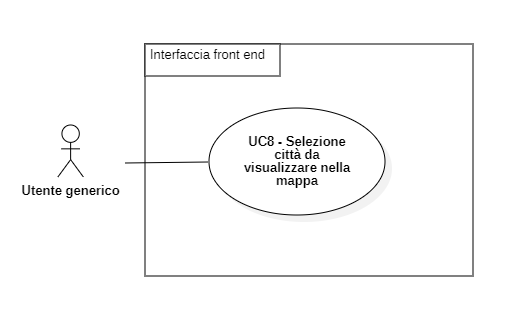
\includegraphics[scale=0.8]{../immagini/attori_casi/UC_8.png}
		\caption{Schema generale selezione della città}
	\end{figure}
\end{center}


\subsubsection{UC8 - Selezione città da visualizzare nella mappa}\label{CasiDUsoCasiDUsoTraUnUtenteEIlFrontEndElencoCasiDUsoUC4SelezioneCittaDaVisualizzareNellaMappa}

\begin{itemize}
	\item \textbf{Attori primari}: utente generico;
	\item \textbf{Descrizione}: l’utente può selezionare la città di cui vuole visualizzare la heat map$_{\scaleto{G}{3pt}}$;
	\item \textbf{Scenario principale}: l’utente seleziona una città tra quelle messe a disposizione;
	\item \textbf{Precondizione}: il sistema dispone di informazioni relative a diverse città;
	\item \textbf{Postcondizione}:  l’utente ha selezionato la città che vuole visualizzare, la heat-map$_{\scaleto{G}{3pt}}$ si aggiorna in base alla scelta fatta.
\end{itemize}
\begin{center}
	\begin{figure}[H]
		\centering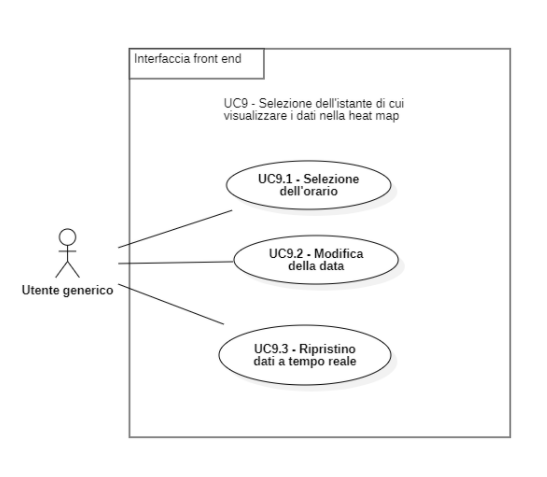
\includegraphics[scale=0.8]{../immagini/attori_casi/UC_9.png}
		\caption{Schema generale della selezione dell'istante di cui visualizzare i dati}
	\end{figure}
\end{center}
\subsubsection{UC9 - Selezione dell’istante di cui visualizzare i dati nella heat map
}\label{CasiDUsoCasiDUsoTraUnUtenteEIlFrontEndElencoCasiDUsoUC5SelezioneDellIstanzeDiCuiVisualizzareIDatiNellaHeatmap}%parzialmente corretto
\begin{center}
	\begin{figure}[H]
		\centering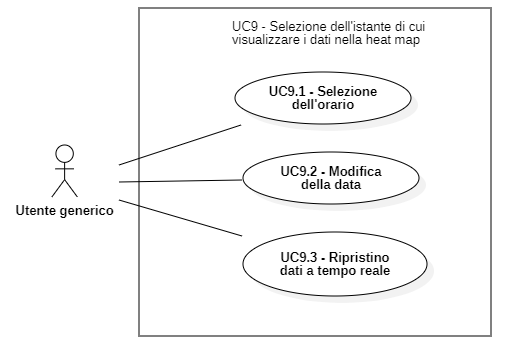
\includegraphics[scale=0.7]{../immagini/attori_casi/UC_9_1_2_3.png}
		\caption{Schema sotto-casi della selezione dell'istante da visualizzare}
	\end{figure}
\end{center}
\begin{itemize}
	\item \textbf{Attori primari}: utente generico;
	\item \textbf{Descrizione}: l’utente, attraverso l’interfaccia del sistema, modifica l’istante di tempo di cui vuole visualizzare i dati;
	\item \textbf{Scenario principale}: attraverso l’interfaccia l’utente può decidere di:
		\begin{enumerate}
			\item Modificare l’orario dei dati da visualizzare (UC9.1, sezione  \ref{CasiDUsoCasiDUsoTraUnUtenteEIlFrontEndElencoCasiDUsoUC51SelezioneDellOrario});
			\item Modificare la data tra quelle disponibili (UC9.2, sezione \ref{CasiDUsoCasiDUsoTraUnUtenteEIlFrontEndElencoCasiDUsoUC52ModificaDellaData});
			\item Ritornare ai dati in tempo reale (UC9.3, sezione \ref{CasiDUsoCasiDUsoTraUnUtenteEIlFrontEndElencoCasiDUsoUC53RipristinoDatiATempoReale}).
		\end{enumerate}
	\item \textbf{Precondizione}: il sistema dispone di informazioni su diversi istanti di tempo;
	\item \textbf{Postcondizione}: l’utente ha selezionato un istante di tempo diverso da quello attuale e visualizza i dati riguardanti ad esso.%insicuro
\end{itemize}

\subsubsection{UC9.1 - Selezione dell’orario}\label{CasiDUsoCasiDUsoTraUnUtenteEIlFrontEndElencoCasiDUsoUC51SelezioneDellOrario}
\begin{itemize}
	\item \textbf{Attori primari}: utente generico;
	\item \textbf{Descrizione}: l’utente seleziona un orario diverso da quello attuale per visualizzare i dati di quel momento;
	\item \textbf{Scenario principale}: l’utente imposta un orario utilizzando l’interfaccia dell’applicazione web;
	\item \textbf{Precondizione}: il sistema ha informazioni riguardanti tutti i diversi orari; %insicuro
	\item \textbf{Postcondizione}: l’orario viene aggiornato e la mappa visualizza i dati della modifica fatta.
\end{itemize}

\subsubsection{UC9.2 - Modifica della data}\label{CasiDUsoCasiDUsoTraUnUtenteEIlFrontEndElencoCasiDUsoUC52ModificaDellaData}
\begin{itemize}
	\item \textbf{Attori primari}: utente generico;
	\item \textbf{Descrizione}: l’utente seleziona una data diversa da quella odierna tra quelle disponibili e visualizza la mappa della data scelta;
	\item \textbf{Scenario principale}: l’utente seleziona una data diversa da quella attuale;
	\item \textbf{Precondizione}: il sistema possiede informazioni su tutte le date fino a quella odierna;
	\item \textbf{Postcondizione}: la data viene aggiornata e l’utente visualizza l’heat map$_{\scaleto{G}{3pt}}$ aggiornata con i dati del giorno selezionato all’orario attuale o all’orario scelto dall’utente stesso, secondo quanto definito nella descrizione dell’UC9.1 (sezione \ref{CasiDUsoCasiDUsoTraUnUtenteEIlFrontEndElencoCasiDUsoUC51SelezioneDellOrario}).
\end{itemize}

\subsubsection{UC9.3 - Ripristino dati a tempo reale}\label{CasiDUsoCasiDUsoTraUnUtenteEIlFrontEndElencoCasiDUsoUC53RipristinoDatiATempoReale}
\begin{itemize}
	\item \textbf{Attori primari}: utente generico;
	\item \textbf{Descrizione}: l’utente sceglie di osservare i dati in tempo reale;
	\item \textbf{Scenario principale}: l’utente preme sul pulsante per il ripristino dei valori attuali di data e ora;
	\item \textbf{Precondizione}: l’utente ha impostato una data e/o un’ora diversa dal valore di quella attuale secondo quanto descritto nell'UC9.1 (sezione \ref{CasiDUsoCasiDUsoTraUnUtenteEIlFrontEndElencoCasiDUsoUC51SelezioneDellOrario}) e nell'UC9.2 (sezione \ref{CasiDUsoCasiDUsoTraUnUtenteEIlFrontEndElencoCasiDUsoUC52ModificaDellaData});
	\item \textbf{Postcondizione}: l’utente visualizza la mappa con i dati in tempo reale.
\end{itemize}


\begin{center}
	\begin{figure}[H]
		\centering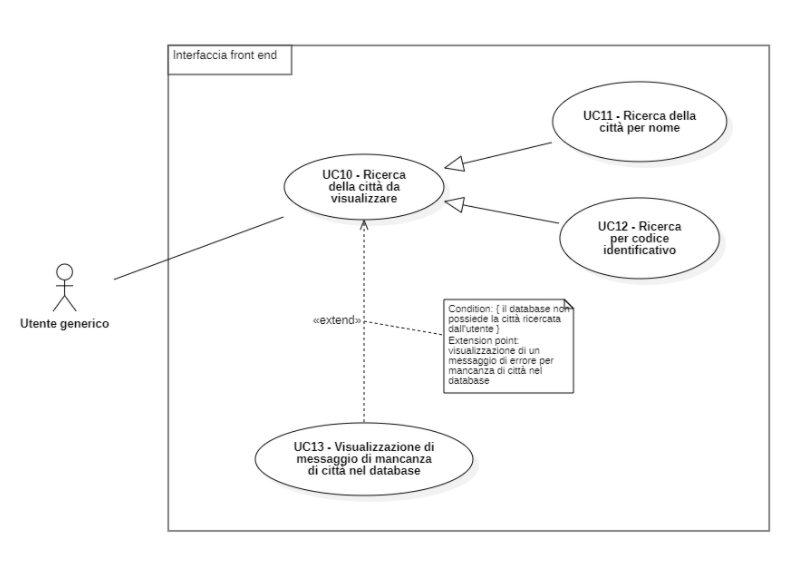
\includegraphics[scale=0.6]{../immagini/attori_casi/UC_10.png}
		\caption{Scherma generale della ricerca ed errori annessi}
	\end{figure}
\end{center}


\subsubsection{UC10 - Ricerca della città da visualizzare}\label{CasiDUsoCasiDUsoTraUnUtenteEIlFrontEndElencoCasiDUsoUC6RicercaDellaCittàDaVisualizzare}

\begin{itemize}
	\item \textbf{Attori primari:} utente generico;
	\item \textbf{Descrizione:} l’utente può ricercare in una barra di ricerca la città da visualizzare;
	\item \textbf{Scenario principale:} l’utente ricerca una città tramite una barra di ricerca;
	\item \textbf{Precondizione:} l’utente ha inserito la città da ricercare;
	\item \textbf{Postcondizione:} l’utente ha inserito la città che vuole cercare e il sistema si aggiorna in base alla ricerca fatta;
	\item \textbf{Generalizzazioni:}
	\begin{itemize}
		\item ricerca della città tramite il suo nome UC11 (sezione \ref{CasiDUsoCasiDUsoTraUnUtenteEIlFrontEndElencoCasiDUsoUC52RicercaDellaCittàDaVisualizzareTramiteNome});
		\item ricerca della città tramite il suo codice UC12 (sezione \ref{CasiDUsoCasiDUsoTraUnUtenteEIlFrontEndElencoCasiDUsoUC61RicercaDellaCittàDaVisualizzareTramiteCodiceIdentificativo}).
	\end{itemize}
	\item \textbf{Estensioni:} l’utente ha ricercato una città non presente nel database, il sistema rileva questo errore e di conseguenza viene visualizzato un messaggio relativo all’errore riscontrato (UC13, sezione \ref{CasiDUsoCasiDUsoTraUnUtenteEIlFrontEndElencoCasiDUsoUC7VisualizzazioneMessaggioDiMancanzaCittàNelDatabase}).
\end{itemize}


\subsubsection{UC11 - Ricerca della città per nome}\label{CasiDUsoCasiDUsoTraUnUtenteEIlFrontEndElencoCasiDUsoUC52RicercaDellaCittàDaVisualizzareTramiteNome}

\begin{itemize}
	\item \textbf{Attori primari:} utente generico;
	\item \textbf{Descrizione:} l’utente ha la possibilità di ricercare la città da visualizzare tramite nome;
	\item \textbf{Scenario principale:} l’utente ricerca la città tramite nome;
	\item \textbf{Precondizione:} l’utente ha inserito il nome della città da ricercare;
	\item \textbf{Postcondizione:} il sistema mostra all’utente il risultato della ricerca effettuata.
\end{itemize}

\subsubsection{UC12 - Ricerca della città per codice identificativo}\label{CasiDUsoCasiDUsoTraUnUtenteEIlFrontEndElencoCasiDUsoUC61RicercaDellaCittàDaVisualizzareTramiteCodiceIdentificativo}
\begin{itemize}
	\item \textbf{Attori primari:} utente generico;
	\item \textbf{Descrizione:} l’utente ha la possibilità di ricercare la città da visualizzare tramite codice identificativo;
	\item \textbf{Scenario principale:} l’utente ricerca la città tramite codice identificativo;
	\item \textbf{Precondizione:} l’utente ha inserito il codice identificativo della città da ricercare;
	\item \textbf{Postcondizione:} il sistema mostra all’utente il risultato della ricerca effettuata.
\end{itemize}



\subsubsection{UC13 - Visualizzazione mancanza città nel database}\label{CasiDUsoCasiDUsoTraUnUtenteEIlFrontEndElencoCasiDUsoUC7VisualizzazioneMessaggioDiMancanzaCittàNelDatabase}

\begin{itemize}
	\item \textbf{Attori primari:} utente generico;
	\item \textbf{Descrizione:} l’utente visualizza un errore per l'inserimento nella barra di ricerca di una città non presente nel database;
	\item \textbf{Scenario principale:}
	\begin{enumerate}
		\item l’operazione di ricerca fallisce;
		\item l’utente visualizza un errore;
		\item l’utente preme "ok" per chiudere il messaggio.
	\end{enumerate}
	\item \textbf{Precondizione:} il front end$_{\scaleto{G}{3pt}}$ effettua un controllo sui dati e non è presente la città ricercata;
	\item \textbf{Postcondizione:} viene visualizzato  un messaggio all’utente per informarlo sul problema.
\end{itemize}

\section{Casi d'uso tra il front end e il back end}\label{CasiDUsoCasiDUsoTraIlFrontEndEIlBackEnd}
%spiegazione sezione

\subsection{Attori dei casi d'uso}\label{CasiDUsoCasiDUsoTraIlFrontEndEIlBackEndAttoriDeiCasiDUso}
%immagine errata
\begin{center}
	\begin{figure}[H]
		\centering
\includegraphics{../immagini/attori_casi/sistema_front_end.png}
		\caption{Attore: Sistema front end}
	\end{figure}
\end{center}
\subsubsection{Attori Primari}\label{CasiDUsoCasiDUsoTraIlFrontEndEIlBackEndAttoriDeiCasiDUsoAttoriPrimari}
\begin{itemize}
	\item \textbf{Sistema front end$_{\scaleto{G}{3pt}}$:} Definisce una parte del sistema sviluppato che interagisce con il sistema back end$_{\scaleto{G}{3pt}}$.
\end{itemize}

\subsection{Elenco casi d'uso}\label{CasiDUsoCasiDUsoTraIlFrontEndEIlBackEndElencoDeiCasiDUso}

\begin{center}
	\begin{figure}[H]
		\centering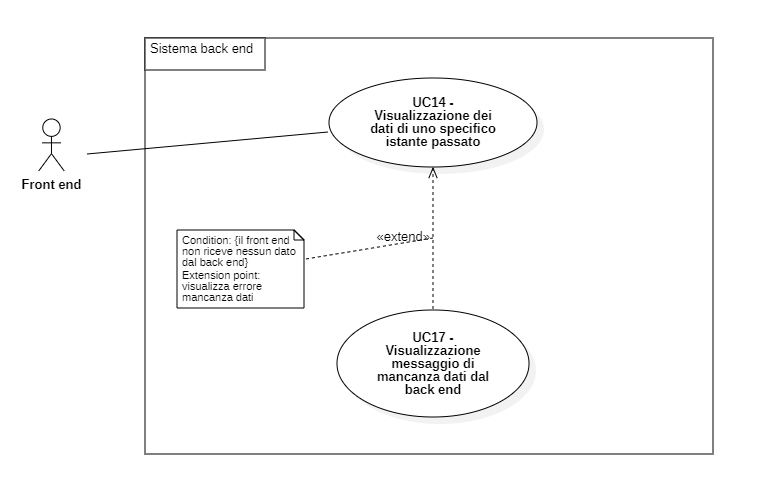
\includegraphics[scale=0.6]{../immagini/attori_casi/UC_14.png}
		\caption{Scherma generale della visualizzazione dei dati di un instante passato}
	\end{figure}
\end{center}

\subsubsection{UC14 - Visualizzazione dei dati di uno specifico istante passato}\label{CasiDUsoCasiDUsoTraIlFrontEndEIlBackEndElencoDeiCasiDUsoUC81VisualizzazioneDeiDatiDiUnoSpecificoIstante}
\begin{itemize}
	\item \textbf{Attori primari}: sistema front end$_{\scaleto{G}{3pt}}$;
	\item \textbf{Descrizione}: il front end$_{\scaleto{G}{3pt}}$ richiede le informazioni relative ad uno specifico istante di tempo passato, vengono visualizzate le informazioni inviate dal back end$_{\scaleto{G}{3pt}}$;
	\item \textbf{Scenario principale}:  il front end$_{\scaleto{G}{3pt}}$ richiede al back end$_{\scaleto{G}{3pt}}$ le informazioni relative all'istante di tempo passato specificato, il back end$_{\scaleto{G}{3pt}}$ invia le informazioni da visualizzare al front end$_{\scaleto{G}{3pt}}$;
	\item \textbf{Precondizione}: l’utente esegue la modifica della data o dell’orario come definito rispettivamente nella descrizione di UC9.2 (sezione \ref{CasiDUsoCasiDUsoTraUnUtenteEIlFrontEndElencoCasiDUsoUC52ModificaDellaData}) e UC9.1 (sezione \ref{CasiDUsoCasiDUsoTraUnUtenteEIlFrontEndElencoCasiDUsoUC51SelezioneDellOrario}) selezionando un istante di tempo precedente a quello attuale;
	\item \textbf{Postcondizione}: il front end$_{\scaleto{G}{3pt}}$ visualizza e riceve le informazioni relative all'istante di tempo passato impostato;
	\item \textbf{Estensione}: il front end$_{\scaleto{G}{3pt}}$ effettua la richiesta al back end$_{\scaleto{G}{3pt}}$ il quale non invia nessun dato nella risposta (UC17, sezione \ref{CasiDUsoCasiDUsoTraIlFrontEndEIlBackEndElencoDeiCasiDUsoUC9VisualizzazioneMessaggioDiMancanzaDatiDalBackEnd}).
\end{itemize}

\begin{center}
	\begin{figure}[H]
		\centering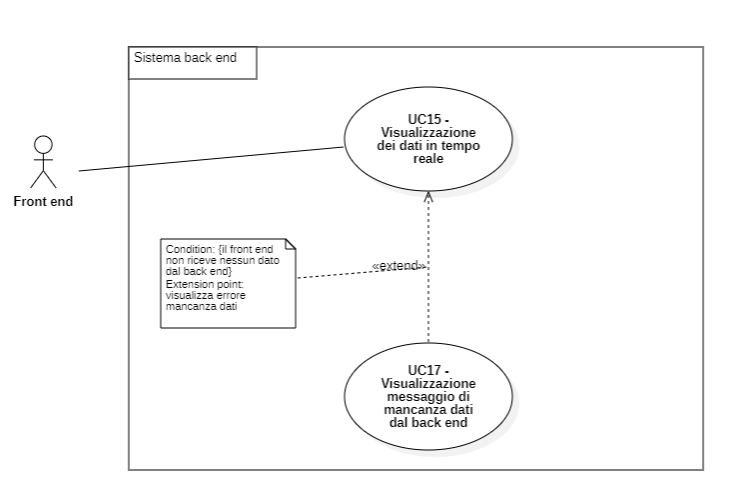
\includegraphics[scale=0.6]{../immagini/attori_casi/UC_15.png}
		\caption{Scherma generale della visualizzazione dei dati in tempo reale}
	\end{figure}
\end{center}


\subsubsection{UC15 - Visualizzazione dei dati in tempo reale}\label{CasiDUsoCasiDUsoTraIlFrontEndEIlBackEndElencoDeiCasiDUsoUC82VisualizzazioneDeiDatiInTempoReale}
\begin{itemize}
	\item \textbf{Attori primari}: sistema front end$_{\scaleto{G}{3pt}}$;
	\item \textbf{Descrizione}: il front end$_{\scaleto{G}{3pt}}$ visualizza i dati reali più recentemente aggiunti;
	\item \textbf{Scenario principale}: il front end$_{\scaleto{G}{3pt}}$ richiede al back end$_{\scaleto{G}{3pt}}$ le informazioni più recentemente aggiunte, una volta ricevute il front end$_{\scaleto{G}{3pt}}$ le visualizza;
	\item \textbf{Precondizione}: viene eseguita la visualizzazione della mappa come definito nell’UC1 (sezione \ref{CasiDUsoCasiDUsoTraUnUtenteEIlFrontEndElencoCasiDUsoUC1VisualizzazioneInformazioniSullaMappa}) o avviene il ripristino dei dati in tempo reale come definito in UC9.3 (sezione \ref{CasiDUsoCasiDUsoTraUnUtenteEIlFrontEndElencoCasiDUsoUC53RipristinoDatiATempoReale});
	\item \textbf{Postcondizione}: il front end$_{\scaleto{G}{3pt}}$ ha ricevuto e visualizzato i dati ed è pronto alla generazione della heat map$_{\scaleto{G}{3pt}}$;
	\item \textbf{Estensione}: il front end$_{\scaleto{G}{3pt}}$ effettua la richiesta al back end$_{\scaleto{G}{3pt}}$ il quale non invia nessun dato nella risposta (UC17, sezione \ref{CasiDUsoCasiDUsoTraIlFrontEndEIlBackEndElencoDeiCasiDUsoUC9VisualizzazioneMessaggioDiMancanzaDatiDalBackEnd}).
\end{itemize}

\begin{center}
	\begin{figure}[H]
		\centering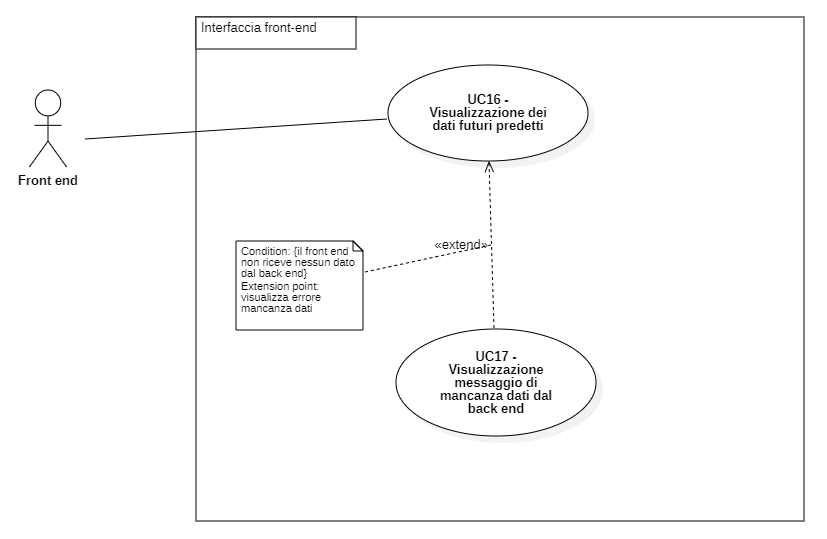
\includegraphics[scale=0.6]{../immagini/attori_casi/UC_16.png}
		\caption{Scherma generale della visualizzazione dei dati futuri predetti}
	\end{figure}
\end{center}


\subsubsection{UC16 - Visualizzazione dei dati futuri predetti}\label{CasiDUsoCasiDUsoTraIlFrontEndEIlBackEndElencoDeiCasiDUsoUC83VisualizzazioneDeiDatiPredetti}
\begin{itemize}
	\item \textbf{Attori primari}: sistema front end$_{\scaleto{G}{3pt}}$;
	\item \textbf{Descrizione}: il front end$_{\scaleto{G}{3pt}}$ richiede i dati i dati della previsione fino al giorno seguente.
	I dati sono ricavati dall’elaborazione, attraverso un modello di machine learning$_{\scaleto{G}{3pt}}$, dei dati reali acquisti. Una volta ricevuti i dati il front end$_{\scaleto{G}{3pt}}$ li può visualizzare;
	\item \textbf{Scenario principale}: il front end$_{\scaleto{G}{3pt}}$ richiede al back end$_{\scaleto{G}{3pt}}$ i dati elaborati dal modello machine learning$_{\scaleto{G}{3pt}}$. Completata la richiesta il front end$_{\scaleto{G}{3pt}}$ visualizzerà i dati inviati dal back end$_{\scaleto{G}{3pt}}$;
	\item \textbf{Precondizione}: le informazioni vengono visualizzate sulla mappa come definito nell’UC1 (sezione \ref{CasiDUsoCasiDUsoTraUnUtenteEIlFrontEndElencoCasiDUsoUC1VisualizzazioneInformazioniSullaMappa}), impostando un orario successivo a quello attuale come descritto nell’UC9.1 (sezione \ref{CasiDUsoCasiDUsoTraUnUtenteEIlFrontEndElencoCasiDUsoUC51SelezioneDellOrario});
	\item \textbf{Postcondizione}: il front end$_{\scaleto{G}{3pt}}$ ha ricevuto e visualizzato i dati ed è pronto alla generazione della heat map$_{\scaleto{G}{3pt}}$;
	\item \textbf{Estensione}: il front end$_{\scaleto{G}{3pt}}$ effettua la richiesta al back end$_{\scaleto{G}{3pt}}$ il quale non invia nessun dato nella risposta (UC17, sezione \ref{CasiDUsoCasiDUsoTraIlFrontEndEIlBackEndElencoDeiCasiDUsoUC9VisualizzazioneMessaggioDiMancanzaDatiDalBackEnd}).
\end{itemize}

\subsubsection{UC17 - Visualizzazione mancanza dati dal back end}\label{CasiDUsoCasiDUsoTraIlFrontEndEIlBackEndElencoDeiCasiDUsoUC9VisualizzazioneMessaggioDiMancanzaDatiDalBackEnd}
\begin{itemize}
	\item \textbf{Attori primari}: sistema front end$_{\scaleto{G}{3pt}}$;
	\item \textbf{Descrizione}: il front end$_{\scaleto{G}{3pt}}$ riceve un errore per la mancanza dati rispetto alla richiesta di visualizzazione effettuata;
	\item \textbf{Scenario principale}:
	\begin{enumerate}
		\item il front end$_{\scaleto{G}{3pt}}$ richiede dei dati specifici al back end$_{\scaleto{G}{3pt}}$;
		\item la risposta ricevuta è un errore;
		\item il front end$_{\scaleto{G}{3pt}}$ ritenta la richiesta di informazioni.
	\end{enumerate}
	\item \textbf{Precondizione}: il front end$_{\scaleto{G}{3pt}}$ effettua una richiesta di dati, il back end$_{\scaleto{G}{3pt}}$ non ha a disposizione i dati richiesti;
	\item \textbf{Postcondizione}: il front end$_{\scaleto{G}{3pt}}$ riceve un errore per la mancanza dei dati da visualizzare.
\end{itemize}

\newpage
\section{Casi d'uso facoltativi tra un utente e il front end}\label{CasiDUsoCasiDUsoFacoltativiTraUnUtenteEIlFrontEnd}
%spiegazione della sezione
L'elenco dei casi d'uso in questa sezione individuano requisiti sviluppabili successivamente a quelli obbligatori descritti nelle sezioni precedenti.
\subsection{Attori dei casi d'uso}
\begin{center}
	\begin{figure}[H]
		\centering
\includegraphics{../immagini/attori_casi/utente_generico.png}
		\caption{Attore: utente generico}
	\end{figure}
\end{center}
\subsubsection{Attori Primari}\label{UFattoriPrimariFac}
\begin{itemize}
	\item \textbf{Utente generico:} definisce l'utente generico che utilizza l'applicazione web.
\end{itemize}

\subsection{Elenco casi d'uso}\label{CasiDUsoCasiDUsoFacoltativiTraUnUtenteEIlFrontEndElencoCasiDUso}



\begin{center}
	\begin{figure}[H]
		\centering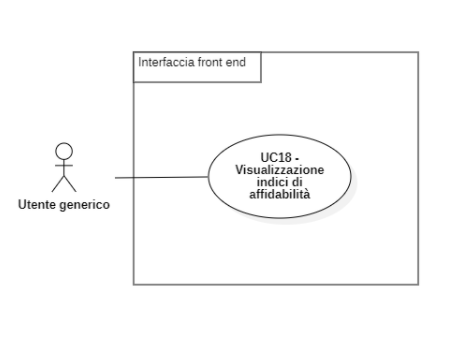
\includegraphics[scale=0.7]{../immagini/attori_casi/UC_18.png}
		\caption{Schema generale della visualizzazione degli indici di affidabilità}
	\end{figure}
\end{center}


\subsubsection{UC18 - Visualizzazione indici di affidabilità}\label{CasiDUsoCasiDUsoFacoltativiTraUnUtenteEIlFrontEndElencoCasiDUsoUC10VisualizzazioneIndiciDiAffidabilita}


\begin{itemize}
	\item \textbf{Attori primari}: utente generico;
	\item \textbf{Descrizione}: l'utente può visualizzare gli indici di affidabilità dei dati reali raccolti e l'indice di affidabilità delle predizioni svolte dal modello di machine learning$_{\scaleto{G}{3pt}}$;
	\item \textbf{Scenario principale}: l'utente attraverso l'interfaccia visualizza gli indici di affidabilità;
	\item \textbf{Precondizione}: il front end$_{\scaleto{G}{3pt}}$ dispone degli indici relativi ai dati reali e predetti;
	\item \textbf{Postcondizione}: l'utente visualizza correttamente gli indici di affidabilità dei dati reali e predetti.
\end{itemize}
\begin{center}
	\begin{figure}[H]
		\centering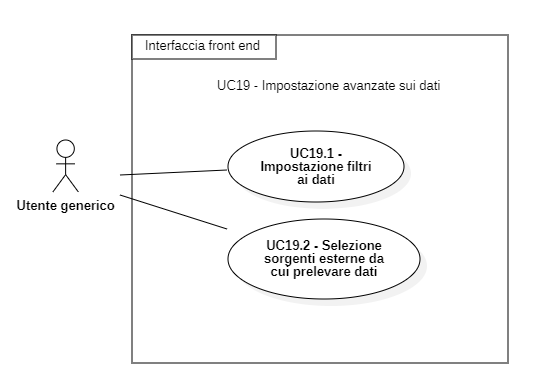
\includegraphics[scale=0.8]{../immagini/attori_casi/UC_19.png}
		\caption{Schema generale delle impostazioni avanzate sui dati}
	\end{figure}
\end{center}
\subsubsection{UC19 - Impostazioni avanzate sui dati}\label{CasiDUsoCasiDUsoFacoltativiTraUnUtenteEIlFrontEndElencoCasiDUsoUC11ImpostazioniAvanzateSuiDati}

\begin{center}
	\begin{figure}[H]
		\centering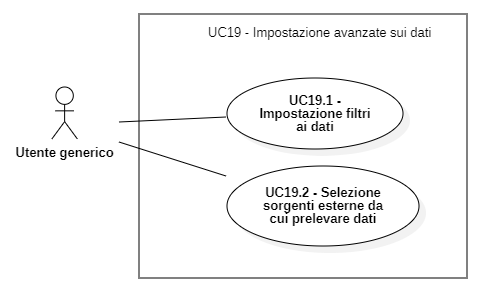
\includegraphics[scale=0.7]{../immagini/attori_casi/UC_19_1_2.png}
		\caption{Schema sotto-casi delle impostazioni avanzate sui dati}
	\end{figure}
\end{center}

\begin{itemize}
	\item \textbf{Attori primari}: utente generico;
	\item \textbf{Descrizione}: l'utente attraverso l'interfaccia del front end$_{\scaleto{G}{3pt}}$ può applicare filtri sui dati e modificare le sorgenti esterne da cui vengono prelevate le informazioni;
	\item \textbf{Scenario principale}: attraverso l'interfaccia l'utente può:
	\begin{itemize}
		\item Applicare filtri ai dati (UC19.1, sezione  \ref{CasiDUsoCasiDUsoFacoltativiTraUnUtenteEIlFrontEndElencoCasiDUsoUC111ApplicazioneFiltriAiDati});
		\item Modificare le sorgenti esterne da cui vengono prelevate le informazioni (UC19.2, sezione \ref{CasiDUsoCasiDUsoFacoltativiTraUnUtenteEIlFrontEndElencoCasiDUsoUC112SelezioneSorgentiEsterneDaCuiPrelevareIDati}).
	\end{itemize}
	\item \textbf{Precondizione}: l'utente visualizza correttamente l'interfaccia e sono disponibili varie sorgenti esterne;
	\item \textbf{Postcondizione}: l'utente applica le impostazioni scelte ai dati e viene aggiornata la mappa di conseguenza.
\end{itemize}

\subsubsection{UC19.1 - Applicazione filtri ai dati}\label{CasiDUsoCasiDUsoFacoltativiTraUnUtenteEIlFrontEndElencoCasiDUsoUC111ApplicazioneFiltriAiDati}
\begin{itemize}
	\item \textbf{Attori primari}: utente generico;
	\item \textbf{Descrizione}: l'utente attraverso l'interfaccia del front end$_{\scaleto{G}{3pt}}$ può applicare filtri sui dati reali e su quelli predetti, modificandone i colori con cui vengono visualizzati nella mappa;
	\item \textbf{Scenario principale}:
	\begin{enumerate}
		\item L'utente può selezionare il colore per i dati reali e/o per quelli predetti;
		\item L'utente conferma i filtri da applicare alla mappa.
	\end{enumerate}
	\item \textbf{Precondizione}: l'utente visualizza correttamente l'interfaccia;
	\item \textbf{Postcondizione}: l'utente applica i filtri ai dati e viene aggiornata la mappa di conseguenza.
\end{itemize}

\subsubsection{UC19.2 - Selezione sorgenti esterne da cui prelevare i dati}\label{CasiDUsoCasiDUsoFacoltativiTraUnUtenteEIlFrontEndElencoCasiDUsoUC112SelezioneSorgentiEsterneDaCuiPrelevareIDati}
\begin{itemize}
	\item \textbf{Attori primari}: utente generico;
	\item \textbf{Descrizione}: l'utente attraverso l'interfaccia del front end$_{\scaleto{G}{3pt}}$ dispone di un menù in cui può selezionare le sorgenti che vuole utilizzare per il reperimento dei dati;
	\item \textbf{Scenario principale}: l'utente decide di selezionare delle diverse sorgenti esterne e indica quelle da cui vuole prelevare informazioni;
	\item \textbf{Precondizione}: l'utente visualizza correttamente l'interfaccia, sono disponibili varie sorgenti esterne;
	\item \textbf{Postcondizione}: l'utente visualizza la mappa con i soli dati delle sorgenti scelte.
\end{itemize}



\begin{center}
	\begin{figure}[H]
		\centering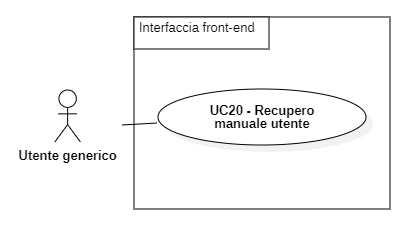
\includegraphics[scale=0.8]{../immagini/attori_casi/UC_20.png}
		\caption{Schema generale recupero manuale utente}
	\end{figure}
\end{center}


\subsubsection{UC20 - Recupero manuale utente}\label{CasiDUsoCasiDUsoFacoltativiTraUnUtenteEIlFrontEndElencoCasiDUsoUC12RecuperoManualeUtente}


\begin{itemize}
	\item \textbf{Attori primari}: utente generico;
	\item \textbf{Descrizione}: l'utente attraverso l'interfaccia del front end$_{\scaleto{G}{3pt}}$ può recuperare il manuale d'uso per informazioni sull'utilizzo dell'applicazione web;
	\item \textbf{Scenario principale}: l'utente seleziona il link al recupero del manuale utente;
	\item \textbf{Precondizione}: il front end$_{\scaleto{G}{3pt}}$ dispone del manuale utente;
	\item \textbf{Postcondizione}: l'utente dispone del manuale utente sul proprio dispositivo e lo può visualizzare.
\end{itemize}


\begin{center}
	\begin{figure}[H]
		\centering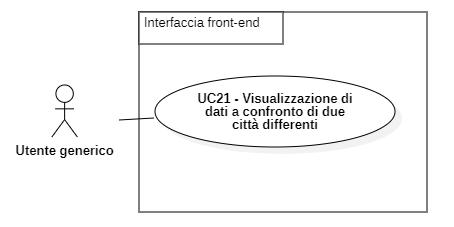
\includegraphics[scale=0.7]{../immagini/attori_casi/UC_21.png}
		\caption{Schema generale visualizzazione delle città a confronto}
	\end{figure}
\end{center}


\subsubsection{UC21 - Visualizzazione di dati a confronto di due città differenti}\label{CasiDUsoCasiDUsoFacoltativiTraUnUtenteEIlFrontEndElencoCasiDUsoUC13VisualizzazioneDiDatiAConfrontoDiDueCittaDifferenti}
\begin{center}
	\begin{figure}[H]
		\centering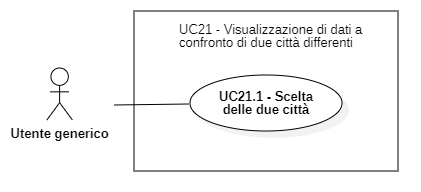
\includegraphics[scale=0.7]{../immagini/attori_casi/UC_21_1.png}
		\caption{Schema sotto-casi della visualizzazione delle città a confronto}
	\end{figure}
\end{center}

\begin{itemize}
	\item \textbf{Attori primari}: utente generico;
	\item \textbf{Descrizione}: l’utente può selezionare due città per poter mettere a confronto i loro dati;
	\item \textbf{Scenario principale}: l’utente seleziona le due città e visualizza i dati a confronto;
	\item \textbf{Precondizione}: il sistema dispone le informazioni riguardanti le città;
	\item \textbf{Postcondizione}: l'utente visualizza i dati di entrambe le città per poterli mettere a confronto.
\end{itemize}

\subsubsection{UC21.1 - Scelta delle due città}
\begin{itemize}
	\item \textbf{Attori primari}: utente generico;
	\item \textbf{Descrizione}: l'utente seleziona le due città da mettere a confronto per la visualizzazione dei dati;
	\item \textbf{Scenario principale}: l’utente seleziona le due città;
	\item \textbf{Precondizione}: il sistema ha informazioni su diverse città;
	\item \textbf{Postcondizione}: l'utente ha scelto le due città da confrontare.
\end{itemize}


\begin{center}
	\begin{figure}[H]
		\centering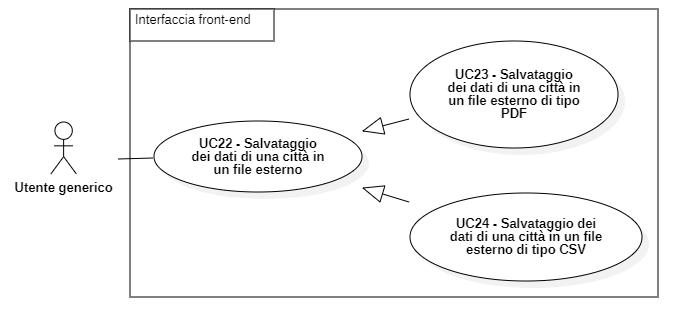
\includegraphics[scale=0.7]{../immagini/attori_casi/UC_22_23_24.png}
		\caption{Schema generale del salvataggio dei dati in un file esterno}
	\end{figure}
\end{center}


\subsubsection{UC22 - Salvataggio dei dati di una città in un file esterno}\label{CasiDUsoCasiDUsoFacoltativiTraUnUtenteEIlFrontEndElencoCasiDUsoUC14SalvataggioDeiDatiDiUnaCittaInUnFileEsterno}


\begin{itemize}
	\item \textbf{Attori primari}: utente generico;
	\item \textbf{Descrizione}: l’utente ha la possibilità di salvare localmente i dati relativi ad una città in un file;
	\item \textbf{Scenario principale}: l’utente salva localmente i dati della città che sta visualizzando;
	\item \textbf{Precondizione}: il sistema dispone delle informazioni riguardanti le città e  l’utente sta visualizzando la heat map$_{\scaleto{G}{3pt}}$ di una città in particolare;
	\item \textbf{Postcondizione}: il sistema ha salvato localmente i dati della città che sta visualizzando.
\end{itemize}

\subsubsection{UC23 - Salvataggio dei dati di una città in un file esterno di tipo PDF}\label{CasiDUsoCasiDUsoFacoltativiTraUnUtenteEIlFrontEndElencoCasiDUsoUC141SalvataggioDeiDatiDiUnaCittaInUnFileEsternoDiTipoPdf}

\begin{itemize}
	\item \textbf{Attori primari}: utente generico;
	\item \textbf{Descrizione}: l’utente può selezionare l’estensione del file in PDF;
	\item \textbf{Scenario principale}: l’utente seleziona l’estensione del file in PDF;
	\item \textbf{Precondizione}: il sistema dispone delle informazioni riguardanti le città e  l’utente sta visualizzando la heat map$_{\scaleto{G}{3pt}}$ di una città in particolare;
	\item \textbf{Postcondizione}: il sistema ha salvato localmente i dati in formato PDF.
\end{itemize}

\subsubsection{UC24 - Salvataggio dei dati di una città in un file esterno di tipo CSV}\label{CasiDUsoCasiDUsoFacoltativiTraUnUtenteEIlFrontEndElencoCasiDUsoUC142SalvataggioDeiDatiDiUnaCittaInUnFileEsternoDiTipoCsv}

\begin{itemize}
	\item \textbf{Attori primari}: utente generico;
	\item \textbf{Descrizione}: l’utente può selezionare l’estensione del file in CSV;
	\item \textbf{Scenario principale}: l’utente seleziona l’estensione del file in CSV;
	\item \textbf{Precondizione}: il sistema dispone delle informazioni riguardanti le città e  l’utente sta visualizzando la heat map$_{\scaleto{G}{3pt}}$ di una città in particolare;
	\item \textbf{Postcondizione}: il sistema ha salvato localmente i dati in formato CSV.
\end{itemize}


\begin{center}
	\begin{figure}[H]
		\centering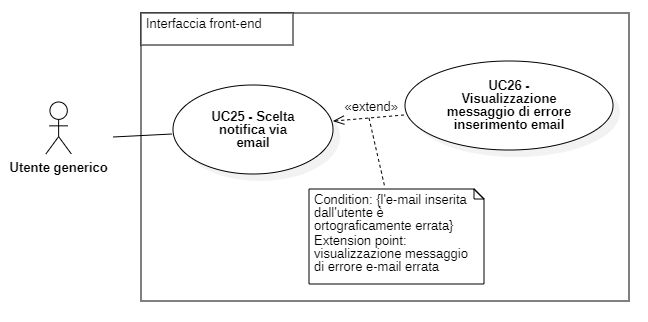
\includegraphics[scale=0.7]{../immagini/attori_casi/UC_25_26.png}
		\caption{Schema generale sulla scelta di notifica via email di una città selezionata}
	\end{figure}
\end{center}

\subsubsection{UC25 - Scelta notifica via e-mail }\label{CasiDUsoCasiDUsoFacoltativiTraUnUtenteEIlFrontEndElencoCasiDUsoUC15NotificaViaEmailDiUnaCittaSelezionata}

\begin{center}
	\begin{figure}[H]
		\centering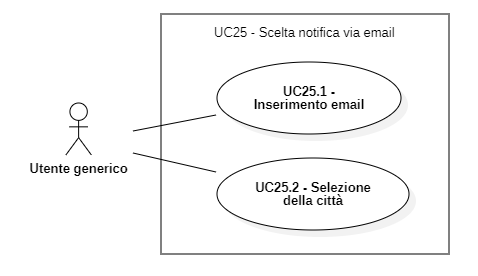
\includegraphics[scale=0.7]{../immagini/attori_casi/UC_25_1_2.png}
		\caption{Schema sotto-casi della scelta di notifica via e-mail}
	\end{figure}
\end{center}

\begin{itemize}
	\item \textbf{Attori primari}: utente generico;
	\item \textbf{Descrizione}: l'utente decide di voler essere notificato via e-mail riguardo gli aggiornamenti relativi ad una determinata città;
	\item \textbf{Scenario principale}:
		\begin{itemize}
			\item inserisce la propria mail (UC25.1, sezione \ref{CasiDUsoCasiDUsoFacoltativiTraUnUtenteEIlFrontEndElencoCasiDUsoUC15.1InserimentoEmail});
			\item seleziona la città di interesse (UC25.2, sezione \ref{CasiDUsoCasiDUsoFacoltativiTraUnUtenteEIlFrontEndElencoCasiDUsoUC15.2SelezioneCitta}).
		\end{itemize}
	\item \textbf{Precondizione}: l'utente sta visualizzando la heat map$_{\scaleto{G}{3pt}}$ e richiede la notifica via e-mail;
	\item \textbf{Postcondizione}: il sistema aggiunge nel database l'e-mail inserita dall'utente e la relativa città di interesse;
	\item \textbf{Estensioni}: il sistema determina che l'e-mail inserita non è valida, di conseguenza viene visualizzato un messaggio d'errore (UC26, sezione \ref{CasiDUsoCasiDUsoFacoltativiTraUnUtenteEIlFrontEndElencoCasiDUsoUC16VisualizzazioneMessaggioDiErroreEmailErrata}).
\end{itemize}

\subsubsection{UC25.1 - Inserimento email}\label{CasiDUsoCasiDUsoFacoltativiTraUnUtenteEIlFrontEndElencoCasiDUsoUC15.1InserimentoEmail}

\begin{itemize}
	\item \textbf{Attori primari}: utente generico;
	\item \textbf{Descrizione}: l'utente inserisce la propria email;
	\item \textbf{Scenario principale}: l'utente inserisce la propria email all'interno del form;
	\item \textbf{Precondizione}: l'utente ha richiesto la notificazione via email;
	\item \textbf{Postcondizione}: il sistema aggiunge nel database l'email inserita dall'utente.
\end{itemize}

\subsubsection{UC25.2 - Selezione della città}\label{CasiDUsoCasiDUsoFacoltativiTraUnUtenteEIlFrontEndElencoCasiDUsoUC15.2SelezioneCitta}

\begin{itemize}
	\item \textbf{Attori primari}: utente generico;
	\item \textbf{Descrizione}: l'utente seleziona la città di suo interesse;
	\item \textbf{Scenario principale}: l'utente seleziona la città di suo interesse;
	\item \textbf{Precondizione}: l'utente ha richiesto la notificazione via email;
	\item \textbf{Postcondizione}: il sistema aggiunge nel database la città selezionata dall'utente per ricevere le notifiche su di essa.
\end{itemize}


\subsubsection{UC26 - Visualizzazione messaggio di errore inserimento email}\label{CasiDUsoCasiDUsoFacoltativiTraUnUtenteEIlFrontEndElencoCasiDUsoUC16VisualizzazioneMessaggioDiErroreEmailErrata}

\begin{itemize}
	\item \textbf{Attori primari}: utente generico;
	\item \textbf{Descrizione}: Il front end$_{\scaleto{G}{3pt}}$ mostra a video un messaggio di errore nell'inserimento della email;
	\item \textbf{Scenario principale}: \begin{itemize}
		\item l'operazione di inserimento email fallisce;
		\item l'utente visualizza il messaggio d'errore;
		\item l'utente clicca il pulsante "ok" per chiudere il messaggio.
	\end{itemize}
	\item \textbf{Precondizione}: l'email inserita non è valida;
	\item \textbf{Postcondizione}: l'utente visualizza un messaggio di errore.
\end{itemize}



\begin{center}
	\begin{figure}[H]
		\centering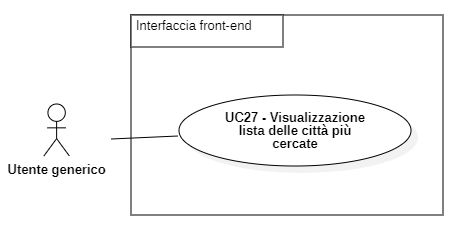
\includegraphics[scale=0.7]{../immagini/attori_casi/UC_27.png}
		\caption{Schema generale della visualizzazione della lista delle città più cercate}
	\end{figure}
\end{center}


\subsubsection{UC27 - Visualizzazione lista delle città più cercate}\label{CasiDUsoCasiDUsoFacoltativiTraUnUtenteEIlFrontEndElencoCasiDUsoUC17VisualizzazioneListaDelleCittaPiuCercate}

\begin{itemize}
	\item \textbf{Attori primari}: utente generico;
	\item \textbf{Descrizione}: l'utente ha la possibilità di visionare la lista delle città più cercate all'interno del sito;
	\item \textbf{Scenario principale}: l'utente visualizza la lista;
	\item \textbf{Precondizione}: il sistema è funzionante e possiede le informazioni riguardanti alle ricerche effettuate dagli utenti;
	\item \textbf{Postcondizione}: il back end$_{\scaleto{G}{3pt}}$ invia al front end$_{\scaleto{G}{3pt}}$ la lista delle città più cercate che verrà visualizzata dall'utente.
\end{itemize}



\begin{center}
	\begin{figure}[H]
		\centering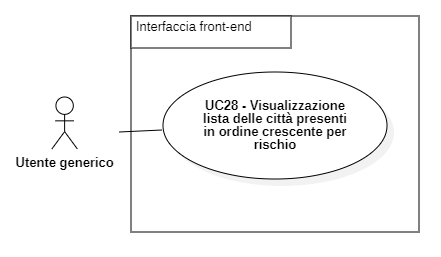
\includegraphics[scale=0.7]{../immagini/attori_casi/UC_28.png}
		\caption{Schema generale visualizzazione delle città in ordine di rischio}
	\end{figure}
\end{center}

\subsubsection{UC28 - Visualizzazione lista delle città presenti in ordine crescente per rischio}\label{CasiDUsoCasiDUsoFacoltativiTraUnUtenteEIlFrontEndElencoCasiDUsoUC18VisualizzazioneListaDelleCittaPresentiInOrdineCrescentePerRischio}


\begin{itemize}
	\item \textbf{Attori primari}: utente generico;
	\item \textbf{Descrizione}: l'utente ha la possibilità di visionare la lista delle città presenti nel sito in ordine crescente per rischio;
	\item \textbf{Scenario principale}: l'utente visualizza la lista;
	\item \textbf{Precondizione}:  il sistema è funzionante e possiede le informazioni riguardanti le città;
	\item \textbf{Postcondizione}: il back end$_{\scaleto{G}{3pt}}$ invia al front end$_{\scaleto{G}{3pt}}$ la lista delle città in ordine crescente per rischio che verrà visualizzata dall'utente.
\end{itemize}
